% Source: perceptron_trick.tex
\begin{notechapter}
\chapter{The Perceptron Trick}\label{ch:perceptron-trick}
\chaptersubtitle{A geometric interpretation}

\section{Mathematical Setup}

We consider binary classification in $\mathbb{R}^2$:

\begin{itemize}
    \item Input point: $\mathbf{x} = (p, q)$ with label $y \in \{-1, +1\}$ \\
    (if $y \in \{0, +1\}$ replace $y$ by $2y-1$)
    \item Augmented vector: $\tilde{\mathbf{x}} = (p, q, 1)$
    \item Parameter vector: $\boldsymbol{\theta} = (w_1, w_2, b)$
    \item Prediction: $\hat{y} = \text{step}
    (\boldsymbol{\theta} \cdot \tilde{\mathbf{x}}) = \text{step}(w_1 p + w_2 q + b)$
    \item Learning rate: $\alpha > 0$
\end{itemize}

\section{Perceptron Update Rule}

The perceptron algorithm updates only on misclassified points:

\[
\boldsymbol{\theta}^{(t+1)} = \boldsymbol{\theta}^{(t)} + \alpha \, y \, \tilde{\mathbf{x}} \quad \text{if} \quad y(\boldsymbol{\theta}^{(t)} \cdot \tilde{\mathbf{x}}) \leq 0
\]

In component form for the 2D case:

\begin{align*}
w_1 &\leftarrow w_1 + \alpha y p \\
w_2 &\leftarrow w_2 + \alpha y q \\
b &\leftarrow b + \alpha y
\end{align*}

Or equivalently as described:

\begin{itemize}
    \item If correctly classified: do nothing
    \item If $\hat{y}=+1$ but $y=-1$: $(w_1, w_2, b) \leftarrow (w_1 - \alpha p, w_2 - \alpha q, b - \alpha)$
    \item If $\hat{y}=-1$ but $y=+1$: $(w_1, w_2, b) \leftarrow (w_1 + \alpha p, w_2 + \alpha q, b + \alpha)$
\end{itemize}

\section{Geometric Interpretation}

\subsection{Decision Boundary and Normal Vector}

The decision boundary is the line:
\[
w_1 x_1 + w_2 x_2 + b = 0
\]

The vector $\mathbf{w} = (w_1, w_2)$ is \textbf{normal} to this line. For any two points $\mathbf{x}_1, \mathbf{x}_2$ on the line:
\[
\mathbf{w} \cdot (\mathbf{x}_1 - \mathbf{x}_2) = 0
\]

The sign of $\mathbf{w} \cdot \mathbf{x} + b$ determines the classification:
\begin{itemize}
    \item $\mathbf{w} \cdot \mathbf{x} + b \geq 0$ → Class $+1$ (positive region)
    \item $\mathbf{w} \cdot \mathbf{x} + b < 0$ → Class $-1$ (negative region)
\end{itemize}

\subsection{Visualization of the Perceptron}

\begin{figure}[H]
\centering
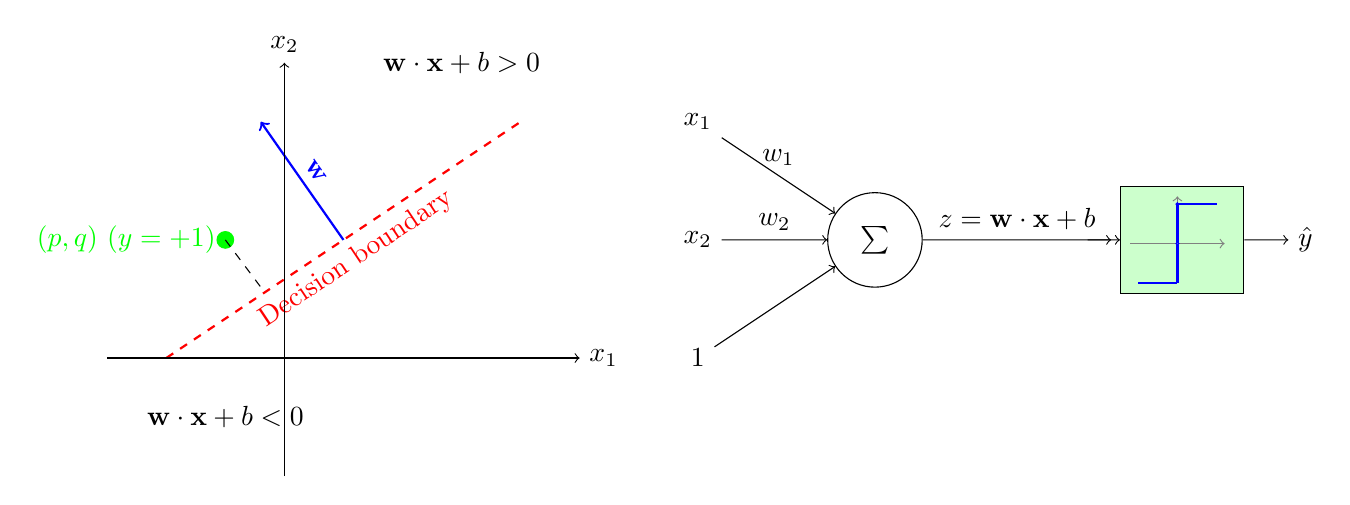
\begin{tikzpicture}[scale=1.5]
    % Decision boundary
    \draw[thick, red, dashed] (-1,0) -- (2,2) node[midway, below, sloped] 
    {Decision boundary};
    
    % Normal vector
    \draw[thick, blue, ->] (0.5,1) -- (-0.2,2) node[midway, above, sloped] 
    {$\mathbf{w}$};
    
    % Positive and negative regions
    \node at (1.5, 2.5) {$\mathbf{w} \cdot \mathbf{x} + b > 0$};
    \node at (-0.5, -0.5) {$\mathbf{w} \cdot \mathbf{x} + b < 0$};
    
    % Coordinate axes
    \draw[->] (-1.5,0) -- (2.5,0) node[right] {$x_1$};
    \draw[->] (0,-1) -- (0,2.5) node[above] {$x_2$};
    
    % A misclassified positive point
    \filldraw[green] (-0.5,1) circle (2pt) node[left] {$(p,q)$ ($y=+1$)};
    
    % Distance to boundary
    \draw[dashed] (-0.5,1) -- (-0.2,0.6);
    
    % Perceptron diagram components
    \node[draw, circle, minimum size=1.2cm] (perc) at (5,1) {$\sum$};
    \node (x1) at (3.5,2) {$x_1$};
    \node (x2) at (3.5,1) {$x_2$};
    \node (bias) at (3.5,0) {$1$};
    
    \draw[->] (x1) -- (perc) node[midway, above] {$w_1$};
    \draw[->] (x2) -- (perc) node[midway, above] {$w_2$};
    \draw[->] (bias) -- (perc);
    
    % Line for the 'z' value before the step function
    \draw[->] (perc.east) -- (7,1) node[midway, above] 
    {$z = \mathbf{w}\cdot\mathbf{x}+b$};
    
    % Node with the step function drawn inside using simple \draw commands (no scope)
    \node[draw, rectangle, minimum width=1.4cm, minimum height=0.8cm,
    fill=green!20, align=center] (step_node) at (7.6, 1) {
        % Use \tikz\draw to embed single drawing commands within standard text flow
        \tikz{\draw[->, thin, gray] (-0.6, 0) -- (0.6, 0);
              \draw[->, thin, gray] (0, -0.1) -- (0, 0.6);
              \draw[thick, blue] (-0.5, -0.5) -- (0, -0.5);      
              \draw[thick, blue] (0, 0.5) -- (0.5, 0.5);   
              \draw[thick, blue] (0, -0.5) -- (0, 0.5);       
              \filldraw[blue] (0, 0.5) circle (0.5pt);
              \draw[blue, fill=white] (0, 0) circle (0.5pt);
        }
    };
    
    % Connect the sum node output to the step node input
    \draw[->] (6.8, 1) -- (step_node.west); 

    % Output from the step node
    \draw[->] (step_node.east) -- (8.5,1) node[right] {$\hat{y}$};
\end{tikzpicture}
\end{figure}

\subsection{Understanding the Boundary Rotation}

When we update $\mathbf{w} \leftarrow \mathbf{w} + \alpha y \mathbf{x}$ and
$b \leftarrow b + \alpha y$, the decision boundary
\textbf{rotate around a fixed point in input space}.\\

\noindent Let's find this pivot point mathematically.

\subsubsection{Derivation of the Pivot Point}

Old boundary equation:
\[
w_1 x_1 + w_2 x_2 + b = 0 \quad \text{(1)}
\]

\noindent New boundary after update:
\[
(w_1 + \alpha y p)x_1 + (w_2 + \alpha y q)x_2 + (b + \alpha y) = 0 
\quad \text{(2)}
\] 
Which can be rewritten as:
\[
w_1 x_1 + w_2 x_2 + b + \alpha y (p x_1 + q x_2 + 1) = 0
\]

\noindent For any point $(x_1, x_2)$ satisfying (1) we have:
\[
\alpha y (p x_1 + q x_2 + 1) = 0
\]

\noindent Since $\alpha y \neq 0$ when updating, we get:
\[
p x_1 + q x_2 + 1 = 0 \quad \text{(3)}
\]
\\
Any point satisfying both (1) and (3) lies on both the old and new boundaries.\\
The intersection of these two lines is the \textbf{pivot point} around which
the boundary rotates.

\subsection{Geometric Interpretation of the Pivot Point}

\subsubsection{Geometric Relationship}

The line $p x_1 + q x_2 + 1 = 0$ has normal vector $\mathbf{n} = (p, q)$. This means:

\begin{itemize}
    \item The line is perpendicular to the vector $(p, q)$
    \item The line is parallel to any vector perpendicular to $(p, q)$
    \item The misclassified point's position vector $(p, q)$ is perpendicular
    to this line
\end{itemize}

To verify: For any two points $\mathbf{x}_a$ and $\mathbf{x}_b$ on line (3), we have:
\[
(p, q) \cdot (\mathbf{x}_a - \mathbf{x}_b) = 0
\]
So $(p, q)$ is perpendicular to the direction of the line.

The pivot point $\mathbf{x}_0 = (x_1^0, x_2^0)$ satisfies:
\[
\begin{cases}
w_1 x_1^0 + w_2 x_2^0 + b = 0 \\
p x_1^0 + q x_2^0 + 1 = 0
\end{cases}
\]

Solving this system gives:
\[
\mathbf{x}_0 = \left( \frac{w_2 - bq}{w_1q - w_2p}, \frac{bp - w_1}{w_1q - w_2p} \right) \quad \text{(when } w_1q \neq w_2p\text{)}
\]

This pivot point has a special property: the vector from $\mathbf{x}_0$ to the misclassified point $\mathbf{x} = (p, q)$ is:
\[
\mathbf{x} - \mathbf{x}_0 = (p - x_1^0, q - x_2^0)
\]
and this vector satisfies that its projection onto the new normal direction $\mathbf{w}_{\text{new}}$ will be positive after the update (for case $y=+1$).

\begin{figure}[H]
\centering
\begin{tikzpicture}[scale=1.2]
    
    % Draw axes
    \draw[->] (-1.5,0) -- (2.5,0) node[right] {$x_1$};
    \draw[->] (0,-0.5) -- (0,2.5) node[above] {$x_2$};
    
    % Original boundary (red)
    \draw[thick, red, dashed] (-2,0.7) -- (4,0.8);
    
    % Line p*x1 + q*x2 + 1 = 0
    \draw[thick, gray!50!black, dashed] (-1.2,1.0) -- (4,0.2);
    
    % Find intersection (pivot point) - approximately (0.5,0.75)
    \coordinate (P) at (0.5,0.75);
    \filldraw[black] (P) circle (2pt) node[below] {$\mathbf{x}_0$};
    
    % Misclassified point (green)
    \coordinate (X) at (0.3,2);
    \filldraw[green] (X) circle (2pt) node[above right] {$\mathbf{x}=(p,q)$};
    
    % Draw vector from pivot to point
    \draw[thick, green, ->] (P) -- (X) node[pos=0.4, rotate=12, right] 
    {$\overrightarrow{\mathbf{x} - \mathbf{x}_0}$};
    
    % Draw position vector of point from origin
    \draw[thick, blue, ->] (0,0) -- (X) node[pos=0.7, rotate=-10, left]
    {$\overrightarrow{ \mathbf{x} } =
    \begin{bmatrix}
    p\\
    q
    \end{bmatrix} $};
    
    % Add labels for the lines
    \node[red, rotate=2] at (-2.0,0.45) {$w_1x_1+w_2x_2+b=0$};
    \node[gray!50!black, rotate=-9] at (-2.0,1.3) {$px_1+qx_2+1=0$};
    
    % Add legend
    \begin{scope}[shift={(3, 1.5)}]
        \draw[thick, red, dashed] (1.5,0) -- (1.9,0);
        \node[right] at (2, 0) {Old boundary};
        
        \draw[thick, gray!50!black, dashed] (1.5,-0.5) -- (1.9,-0.5);
        \node[right] at (2, -0.5) {$px_1+qx_2+1=0$};
        
        \filldraw[black] (1.8,-1) circle (2pt);
        \node[right] at (2, -1) {Pivot point $\mathbf{x}_0$};
        
        \draw[thick, green, ->] (1.5, -1.5) -- (1.9, -1.5);
        \node[right] at (2, -1.5) {\color{green}
        $\overrightarrow{\mathbf{x}-\mathbf{x}_0}$};
    \end{scope}

\end{tikzpicture}
\caption{The pivot point $\mathbf{x}_0$ lies at the intersection of the old boundary and the line $p x_1 + q x_2 + 1 = 0$. The vector $\mathbf{x}-\mathbf{x}_0$ plays a key role in the update.}
\end{figure}

\begin{figure}[H]
\centering
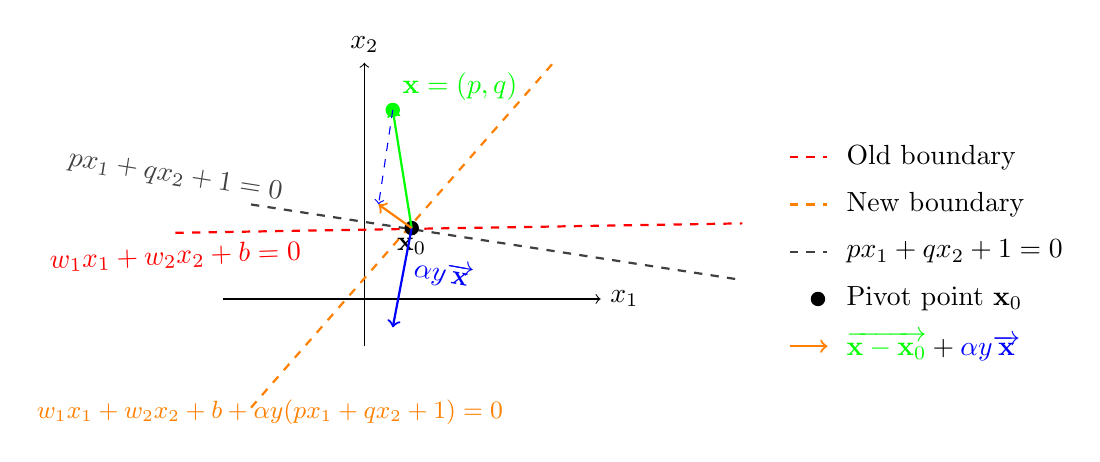
\begin{tikzpicture}[scale=1.2]
    
    % Draw axes
    \draw[->] (-1.5,0) -- (2.5,0) node[right] {$x_1$};
    \draw[->] (0,-0.5) -- (0,2.5) node[above] {$x_2$};
    
    % Original boundary (red)
    \draw[thick, red, dashed] (-2,0.7) -- (4,0.8);
    
    % Line p*x1 + q*x2 + 1 = 0
    \draw[thick, gray!50!black, dashed] (-1.2,1.0) -- (4,0.2);
    
    % New boundery (orange)
    \draw[thick, orange, dashed] (-1.2,-1.15) -- (2,2.5);

    % Find intersection (pivot point) - approximately (0.5,0.75)
    \coordinate (P) at (0.5,0.75);
    \filldraw[black] (P) circle (2pt) node[below] {$\mathbf{x}_0$};
    
    % Misclassified point (green)
    \coordinate (X) at (0.3,2);
    \filldraw[green] (X) circle (2pt) node[above right] {$\mathbf{x}=(p,q)$};
    
    % Draw vector from pivot to point
    \draw[thick, green, ->] (P) -- (X) node[pos=0.4, rotate=12, right]{};
    
    % Draw scaled vector x from pivot point
    \draw[thick, blue, ->] (0.5,0.75) -- (0.3, -0.3)
    node[pos=0.4, rotate=-10, right]
    {$\alpha y \overrightarrow{ \mathbf{x} }$};
    
    \draw[thin, dashed, blue, ->] (X) -- (0.15, 1)
    node[rotate=-20, midway, left] {};

    \draw[thick, orange, ->] (P) -- (0.15, 1) {};
    
    % Add labels for the lines
    \node[red, rotate=2] at (-2.0,0.45) {$w_1x_1+w_2x_2+b=0$};
    \node[gray!50!black, rotate=-9] at (-2.0,1.3) {$px_1+qx_2+1=0$};
    \node[orange, rotate=0, font=\small] at (-1.0,-1.2) {$w_1x_1+w_2x_2+b +
    \alpha y (px_1+qx_2+1)=0$};
    
    % Add legend
    \begin{scope}[shift={(3, 1.5)}]
        \draw[thick, red, dashed] (1.5,0) -- (1.9,0);
        \node[right] at (2, 0) {Old boundary};

        \draw[thick, orange, dashed] (1.5,-0.5) -- (1.9,-0.5);
        \node[right] at (2, -0.5) {New boundary};
        
        \draw[thick, gray!50!black, dashed] (1.5,-1) -- (1.9,-1);
        \node[right] at (2, -1) {$px_1+qx_2+1=0$};
        
        \filldraw[black] (1.8,-1.5) circle (2pt);
        \node[right] at (2, -1.5) {Pivot point $\mathbf{x}_0$};
        
        \draw[thick, orange, ->] (1.5, -2) -- (1.9, -2);
        \node[right] at (2, -2) { \color{green}
        $\overrightarrow{\mathbf{x} - \mathbf{x}_0}
        \color{black} + \color{blue}
        \alpha y \overrightarrow{ \mathbf{x} }$};
    \end{scope}

\end{tikzpicture}
\end{figure}


\begin{figure}[H]
\centering
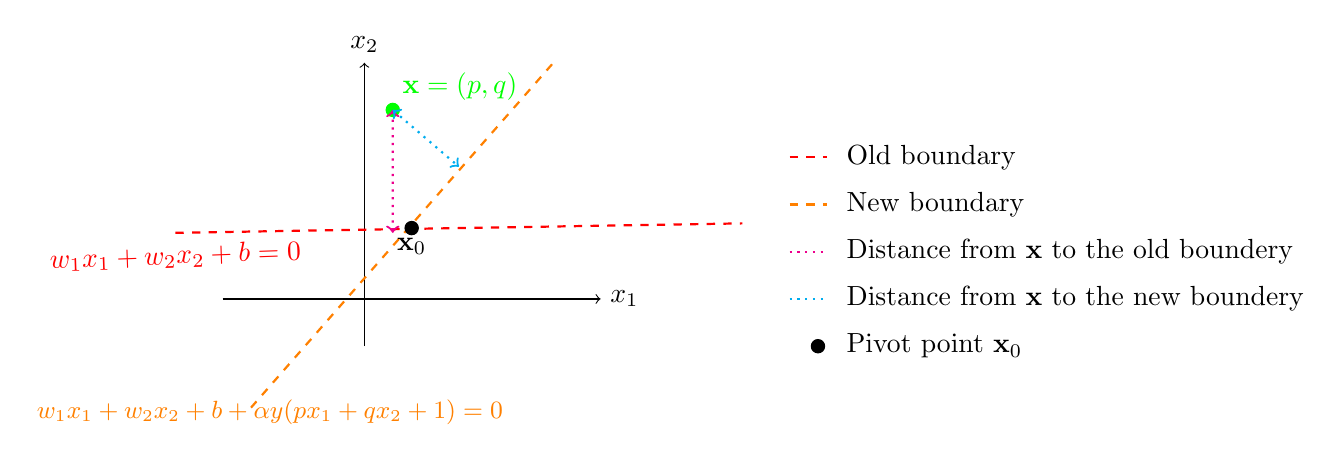
\begin{tikzpicture}[scale=1.2]
    
    % Draw axes
    \draw[->] (-1.5,0) -- (2.5,0) node[right] {$x_1$};
    \draw[->] (0,-0.5) -- (0,2.5) node[above] {$x_2$};
    
    % Original boundary (red)
    \draw[thick, red, dashed] (-2,0.7) -- (4,0.8);
    
    % New boundery (orange)
    \draw[thick, orange, dashed] (-1.2,-1.15) -- (2,2.5);

    % Find intersection (pivot point) - approximately (0.5,0.75)
    \coordinate (P) at (0.5,0.75);
    \filldraw[black] (P) circle (2pt) node[below] {$\mathbf{x}_0$};
    
    % Misclassified point (green)
    \coordinate (X) at (0.3,2);
    \filldraw[green] (X) circle (2pt) node[above right] {$\mathbf{x}=(p,q)$};
    
    % Draw projection on old boundery
    \draw[thick, magenta, dotted, <->] (X) -- (0.3,0.7) node[pos=0.4, rotate=12, right]{};
    
    % Draw projection on new boundery
    \draw[thick, cyan, dotted, <->] (X) -- (1,1.4) node[pos=0.4, rotate=12, right]{};
    
    % Add labels for the lines
    \node[red, rotate=2] at (-2.0,0.45) {$w_1x_1+w_2x_2+b=0$};
    \node[orange, rotate=0, font=\small] at (-1.0,-1.2) {$w_1x_1+w_2x_2+b +
    \alpha y (px_1+qx_2+1)=0$};
    
    % Add legend
    \begin{scope}[shift={(3, 1.5)}]
        \draw[thick, red, dashed] (1.5,0) -- (1.9,0);
        \node[right] at (2, 0) {Old boundary};

        \draw[thick, orange, dashed] (1.5,-0.5) -- (1.9,-0.5);
        \node[right] at (2, -0.5) {New boundary};
        
        \draw[thick, magenta, dotted] (1.5,-1) -- (1.9,-1);
        \node[right] at (2, -1) {Distance from $\mathbf{x}$ to the old boundery};
        
        \draw[thick, cyan, dotted] (1.5,-1.5) -- (1.9,-1.5);
        \node[right] at (2, -1.5) {Distance from $\mathbf{x}$ to the new boundery};
        
        \filldraw[black] (1.8,-2) circle (2pt);
        \node[right] at (2, -2) {Pivot point $\mathbf{x}_0$};
        
    \end{scope}

\end{tikzpicture}
\end{figure}

\subsubsection{Key Insight About the Geometry}

The line $p x_1 + q x_2 + 1 = 0$ is perpendicular to the position vector $\mathbf{x} = (p, q)$, but it does \textbf{not} pass through $\mathbf{x}$:

\begin{itemize}
    \item The line $p x_1 + q x_2 + 1 = 0$ has normal vector $(p, q)$
    \item Therefore, the line is perpendicular to $(p, q)$
    \item The dot product $(p, q) \cdot \mathbf{x} = p^2 + q^2 > 0$ for $\mathbf{x} = (p, q)$
    \item So $\mathbf{x}$ is not on this line (unless $p^2 + q^2 = -1$, which is impossible)
\end{itemize}

The pivot point $\mathbf{x}_0$ is special because:
\[
p x_1^0 + q x_2^0 = -1
\]
So the projection of $\mathbf{x}_0$ onto $(p, q)$ has length $-1/\|(p, q)\|$, while $\mathbf{x}$ itself projects to $\|(p, q)\|$.
\subsubsection{Geometric Interpretation of the Pivot Point}

Equation (3) is interesting: it represents a line passing through the
point $(-\frac{1}{p}, 0)$ and $(-1/p, -1/q)$.\\
More importantly, this line is
\textbf{perpendicular to the misclassified point's position vector} $(p, q)$
when ignoring the constant term.

The pivot point $\mathbf{x}_0 = (x_1^0, x_2^0)$ satisfies:
\[
\begin{cases}
w_1 x_1^0 + w_2 x_2^0 + b = 0 \\
p x_1^0 + q x_2^0 + 1 = 0
\end{cases}
\]

Solving this system gives:
\[
\mathbf{x}_0 = \left( \frac{w_2 - bq}{w_1q - w_2p}, \frac{bp - w_1}{w_1q - w_2p}
\right) \quad \text{(when } w_1q \neq w_2p\text{)}
\]

\begin{figure}[H]
\centering
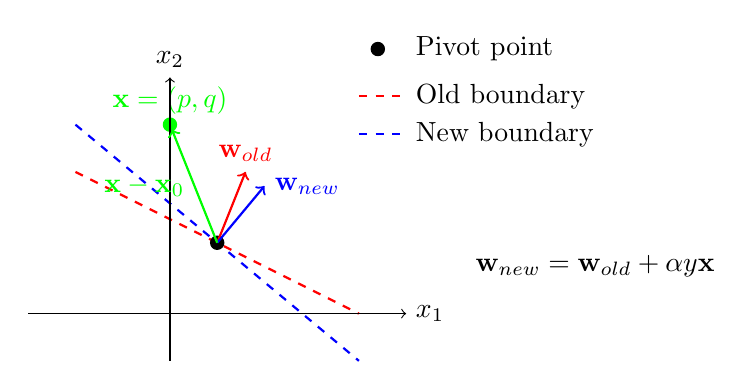
\begin{tikzpicture}[scale=1.2]
    
    % --- Main Diagram Elements ---
    
    % Original boundary
    \draw[thick, red, dashed] (-1,1.5) -- (2,0);
    
    % New boundary
    \draw[thick, blue, dashed] (-1,2) -- (2,-0.5);
    
    % Intersection point (pivot)
    \filldraw[black] (0.5,0.75) circle (2pt) node[above right] {};
    
    % Misclassified point
    \filldraw[green] (0,2) circle (2pt) node[above] {$\mathbf{x}=(p,q)$};
    
    % Normal vectors
    \draw[thick, red, ->] (0.5,0.75) -- (0.8,1.5) node[right, above] {$\mathbf{w}_{\text{old}}$};
    \draw[thick, blue, ->] (0.5,0.75) -- (1.0,1.35) node[right] {$\mathbf{w}_{\text{new}}$};
    
    % Coordinate axes
    \draw[->] (-1.5,0) -- (2.5,0) node[right] {$x_1$};
    \draw[->] (0,-0.5) -- (0,2.5) node[above] {$x_2$};
    
    % Distance vectors
    \draw[->, thick, green] (0.5,0.75) -- (0.02,1.95) node[midway, left] {$\mathbf{x} - \mathbf{x}_0$};
    
    \node at (4.5, 0.5) {$\mathbf{w}_{\text{new}} = \mathbf{w}_{\text{old}} + \alpha y \mathbf{x}$};

    % --- Manual Legend ---
    \begin{scope}[shift={(2.0, 2.3)}] % Adjust the shift coordinates to position the legend box
        \draw[thick, red, dashed] (0,0) -- (0.5,0);
        \node[right] at (0.5, 0) {Old boundary};
        
        \draw[thick, blue, dashed] (0,-0.4) -- (0.5,-0.4);
        \node[right] at (0.5, -0.4) {New boundary};

        \filldraw[black] (0.2,0.5) circle (2pt) (0,-1);
        \node[right] at (0.5, 0.5) {Pivot point};
    \end{scope}

\end{tikzpicture}
\caption{Boundary rotation around a pivot point when $\mathbf{w}$ is updated.}
\end{figure}

\subsection{Case Analysis}

\subsubsection{Case 1: Misclassified Positive ($y=+1$, $\hat{y}=-1$)}

Point is on negative side: $\mathbf{w} \cdot \mathbf{x} + b < 0$.

Update: $\mathbf{w} \leftarrow \mathbf{w} + \alpha \mathbf{x}$, $b \leftarrow b + \alpha$.

Effect: The normal rotates \textbf{toward} the misclassified point, and the boundary shifts to include the point in the positive region.

New dot product:
\[
\mathbf{w}_{\text{new}} \cdot \mathbf{x} + b_{\text{new}} = (\mathbf{w} + \alpha \mathbf{x}) \cdot \mathbf{x} + (b + \alpha) = (\mathbf{w} \cdot \mathbf{x} + b) + \alpha(\|\mathbf{x}\|^2 + 1) > \mathbf{w} \cdot \mathbf{x} + b
\]

\subsubsection{Case 2: Misclassified Negative ($y=-1$, $\hat{y}=+1$)}

Point is on positive side: $\mathbf{w} \cdot \mathbf{x} + b \geq 0$.

Update: $\mathbf{w} \leftarrow \mathbf{w} - \alpha \mathbf{x}$, $b \leftarrow b - \alpha$.

Effect: The normal rotates \textbf{away} from the misclassified point.

New dot product:
\[
\mathbf{w}_{\text{new}} \cdot \mathbf{x} + b_{\text{new}} = (\mathbf{w} - \alpha \mathbf{x}) \cdot \mathbf{x} + (b - \alpha) = (\mathbf{w} \cdot \mathbf{x} + b) - \alpha(\|\mathbf{x}\|^2 + 1) < \mathbf{w} \cdot \mathbf{x} + b
\]

\section{Complete Algorithm}

\begin{figure}[H]
\centering
\begin{tikzpicture}
    \node[draw, rectangle, rounded corners, minimum width=13cm, minimum height=4cm] (box)
    at (2.5,-0.9) {};
    
    \node[draw, ellipse, fill=blue!20] (init) at (0, 2) {Initialize $\mathbf{w}, b$};
    \node[draw, ellipse, fill=yellow!20] (select) at (0, 0) {Select point
    $(\mathbf{x}_i, y_i)$};
    \node[draw, ellipse, fill=green!20] (compute) at (0, -2) {Compute
    $z = \mathbf{w}\cdot\mathbf{x}_i + b$};
    

    \node[draw, diamond, aspect=2, fill=red!20] (decision) at (6, -2) {Correct?};
    \node[draw, ellipse, fill=orange!20, align=center] (update) at (6, -5) {Update:\\ 
    $\mathbf{w} \leftarrow \mathbf{w} + \alpha y_i \mathbf{x}_i$\\ 
    $b \leftarrow b + \alpha y_i$};
    
    \draw[->] (init) -- (select);
    \draw[->] (select) -- (compute);
    \draw[->] (compute) -- (decision);
    \draw[->] (decision) -- node[right] {No} (update);
    \draw[->] (decision.east) -- ++(0.5,0) |- node[right] {Yes} (select.east);
    \draw[->] (update.south) |- ++(0,-0.5) -| (compute.south);
    
    \node at (6.5, 1.5) {Repeat until all points correctly classified};
\end{tikzpicture}
\caption{Perceptron algorithm flowchart.}
\end{figure}

\section{Key Insights}

\begin{enumerate}
    \item The perceptron update can be viewed as rotating the decision boundary's normal vector and shifting the boundary.
    
    \item The "center of rotation" is not fixed at the origin but rather at the intersection point of the old boundary and the line $p x_1 + q x_2 + 1 = 0$.
    
    \item The update $\mathbf{w} \leftarrow \mathbf{w} + \alpha y \mathbf{x}$ changes both the \textbf{direction} (slope) and \textbf{position} of the boundary.
    
    \item For linearly separable data, this algorithm is guaranteed to converge to a separating hyperplane (Perceptron Convergence Theorem).
\end{enumerate}



\subsection{Geometric Interpretation of Adding Equations}

There's a deep geometric insight here: \textbf{Adding a multiple of one line's equation to another line's equation rotates the first line around their intersection point}.

Let's formalize this. Consider two lines:
\[
\begin{aligned}
L_1:& \quad w_1 x_1 + w_2 x_2 + b = 0 \\
L_2:& \quad p x_1 + q x_2 + 1 = 0
\end{aligned}
\]

Their intersection point $\mathbf{x}_0 = (x_1^0, x_2^0)$ satisfies both equations:
\[
\begin{cases}
w_1 x_1^0 + w_2 x_2^0 + b = 0 \\
p x_1^0 + q x_2^0 + 1 = 0
\end{cases}
\]

Now create a new line $L_3$ by adding $\alpha y$ times $L_2$ to $L_1$:
\[
L_3: \quad (w_1 + \alpha y p)x_1 + (w_2 + \alpha y q)x_2 + (b + \alpha y) = 0
\]

\textbf{Key observation:} $\mathbf{x}_0$ also lies on $L_3$ because:
\[
(w_1 + \alpha y p)x_1^0 + (w_2 + \alpha y q)x_2^0 + (b + \alpha y)
= (w_1 x_1^0 + w_2 x_2^0 + b) + \alpha y (p x_1^0 + q x_2^0 + 1) = 0 + \alpha y \cdot 0 = 0
\]

So $L_1$, $L_2$, and $L_3$ all pass through $\mathbf{x}_0$. The perceptron update transforms $L_1$ into $L_3$ by rotating it around the fixed pivot $\mathbf{x}_0$.

\begin{figure}[H]
\centering
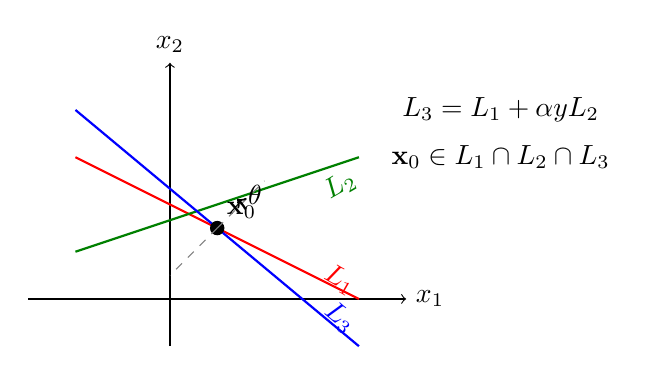
\begin{tikzpicture}[scale=1.2]
    
    % Draw axes
    \draw[->] (-1.5,0) -- (2.5,0) node[right] {$x_1$};
    \draw[->] (0,-0.5) -- (0,2.5) node[above] {$x_2$};
    
    % Original boundary L1 (red)
    \draw[thick, red] (-1,1.5) -- (2,0);
    \node[red, rotate=-30] at (1.8,0.2) {$L_1$};
    
    % Line L2 (green)
    \draw[thick, green!50!black] (-1,0.5) -- (2,1.5);
    \node[green!50!black, rotate=30] at (1.8,1.2) {$L_2$};
    
    % New boundary L3 (blue) - rotated version of L1
    \draw[thick, blue] (-1,2) -- (2,-0.5);
    \node[blue, rotate=-40] at (1.8,-0.2) {$L_3$};
    
    % Intersection point (pivot)
    \coordinate (P) at (0.5,0.75);
    \filldraw[black] (P) circle (2pt) node[above right] {$\mathbf{x}_0$};
    
    % Show that all lines pass through P
    \draw[dashed, gray] (P) -- ++(0.5,0.5);
    \draw[dashed, gray] (P) -- ++(-0.5,-0.5);
    
    % Angles to show rotation
    \draw[->, thick] (0.8,0.95) arc (30:50:0.4);
    \node at (0.9,1.1) {$\theta$};
    
    % Add the mathematical relationship
    \node at (3.5, 2) {$L_3 = L_1 + \alpha y L_2$};
    \node at (3.5, 1.5) {$\mathbf{x}_0 \in L_1 \cap L_2 \cap L_3$};

\end{tikzpicture}
\caption{$L_3$ is obtained by adding $\alpha y$ times $L_2$ to $L_1$, which rotates $L_1$ around their intersection $\mathbf{x}_0$.}
\end{figure}

\subsubsection{Why This Represents Rotation}

For any point $\mathbf{x}$ on $L_1$ but not equal to $\mathbf{x}_0$, let $\mathbf{v} = \mathbf{x} - \mathbf{x}_0$. Since $\mathbf{x}$ is on $L_1$:
\[
w_1 x_1 + w_2 x_2 + b = 0
\]
But $\mathbf{x}_0$ also satisfies this, so:
\[
w_1 (x_1^0 + v_1) + w_2 (x_2^0 + v_2) + b = (w_1 x_1^0 + w_2 x_2^0 + b) + (w_1 v_1 + w_2 v_2) = 0
\]
Thus $w_1 v_1 + w_2 v_2 = 0$, meaning $\mathbf{v}$ is perpendicular to $\mathbf{w}$.

For the new line $L_3$, the normal vector is $\mathbf{w}_{\text{new}} = \mathbf{w} + \alpha y (p, q)$. The angle change $\theta$ satisfies:
\[
\cos\theta = \frac{\mathbf{w} \cdot \mathbf{w}_{\text{new}}}{\|\mathbf{w}\| \|\mathbf{w}_{\text{new}}\|}
\]

Since all lines pass through $\mathbf{x}_0$, $L_3$ is indeed a rotation of $L_1$ around $\mathbf{x}_0$.

\subsubsection{Connection to the Perceptron Update}

In the perceptron trick:
\begin{itemize}
    \item $L_1$ is the current decision boundary: $w_1 x_1 + w_2 x_2 + b = 0$
    \item $L_2$ comes from the misclassified point: $p x_1 + q x_2 + 1 = 0$
    \item The update creates $L_3$: $(w_1 + \alpha y p)x_1 + (w_2 + \alpha y q)x_2 + (b + \alpha y) = 0$
\end{itemize}

The amount of rotation depends on $\alpha y$ and the angle between $\mathbf{w}$ and $(p, q)$. The sign of $y$ determines whether we rotate toward or away from the misclassified point.

\subsection{Point-to-Line Distance and the Normal Vector}

You've identified a crucial relationship: \textbf{The distance from a point to a line is indeed a function of the line's normal vector}. 

For a line defined by $w_1x_1 + w_2x_2 + b = 0$ with normal vector $\mathbf{w} = (w_1, w_2)$, the signed distance from a point $\mathbf{x} = (p, q)$ to the line is:

\[
d(\mathbf{x}) = \frac{w_1p + w_2q + b}{\|\mathbf{w}\|} = \frac{\mathbf{w} \cdot \mathbf{x} + b}{\|\mathbf{w}\|}
\]

\subsubsection{Geometric Interpretation}

The numerator $\mathbf{w} \cdot \mathbf{x} + b$ represents:
\begin{itemize}
    \item The \textbf{scaled distance} from the point to the line
    \item The \textbf{sign} indicates which side of the line the point is on
    \item Positive: point is on the same side as the normal vector $\mathbf{w}$ points
    \item Negative: point is on the opposite side
    \item Zero: point lies exactly on the line
\end{itemize}

The denominator $\|\mathbf{w}\|$ normalizes this to the actual Euclidean distance.

\begin{figure}[H]
\centering
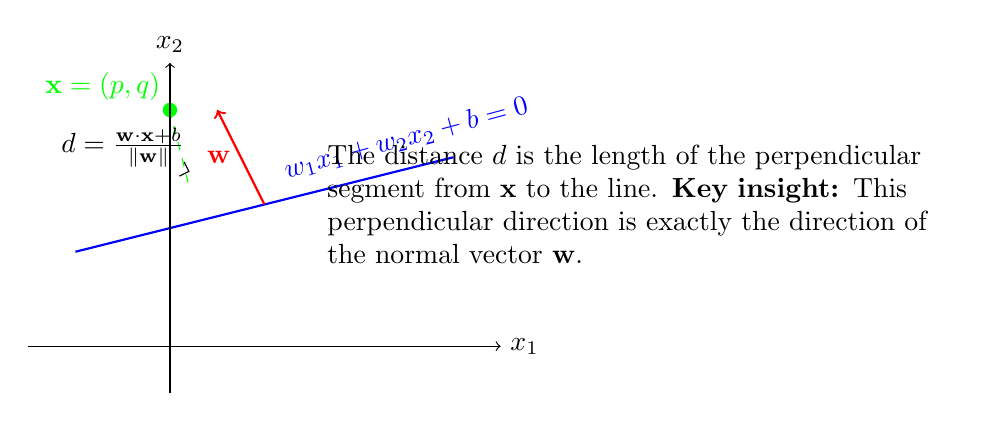
\begin{tikzpicture}[scale=1.2]
    % Draw the line
    \draw[thick, blue] (-1,1) -- (3,2);
    \node[blue, rotate=15] at (2.5,2.2) {$w_1x_1 + w_2x_2 + b = 0$};
    
    % Draw the normal vector
    \draw[thick, red, ->] (1,1.5) -- (0.5,2.5) node[midway, left] {$\mathbf{w}$};
    
    % Draw a point
    \filldraw[green] (0,2.5) circle (2pt) node[above left] {$\mathbf{x} = (p,q)$};
    
    % Draw the distance (perpendicular from point to line)
    \draw[dashed, green] (0,2.5) -- (0.2,1.7);
    
    % Label the distance
    \node at (-0.5,2.1) {$d = \frac{\mathbf{w} \cdot \mathbf{x} + b}{\|\mathbf{w}\|}$};
    
    % Draw axes
    \draw[->] (-1.5,0) -- (3.5,0) node[right] {$x_1$};
    \draw[->] (0,-0.5) -- (0,3) node[above] {$x_2$};
    
    % Add a right angle symbol
    \draw (0.1,1.8) -- (0.2,1.85) -- (0.15,1.95);
    
    % Add explanation
    \node[text width=8cm, align=left] at (5,1.5) {
        The distance $d$ is the length of the perpendicular segment from $\mathbf{x}$ to the line.
        \textbf{Key insight:} This perpendicular direction is exactly the direction of the normal vector $\mathbf{w}$.
    };
    
\end{tikzpicture}
\caption{Point-to-line distance is measured along the direction of the normal vector $\mathbf{w}$.}
\end{figure}

\subsubsection{Connection to the Perceptron Trick}

The perceptron trick fundamentally manipulates this distance function. Consider a misclassified point $\mathbf{x}$ with true label $y$:

\begin{itemize}
    \item If $\hat{y} = +1$ but $y = -1$, then $\mathbf{w} \cdot \mathbf{x} + b \geq 0$ but should be $< 0$
    \item The update $\mathbf{w} \leftarrow \mathbf{w} - \alpha \mathbf{x}$, $b \leftarrow b - \alpha$ changes the signed distance to:
    \[
    \mathbf{w}_{\text{new}} \cdot \mathbf{x} + b_{\text{new}} = (\mathbf{w} \cdot \mathbf{x} + b) - \alpha(\|\mathbf{x}\|^2 + 1)
    \]
    This \textbf{decreases} the (signed) distance, potentially making it negative
    
    \item If $\hat{y} = -1$ but $y = +1$, then $\mathbf{w} \cdot \mathbf{x} + b < 0$ but should be $\geq 0$
    \item The update $\mathbf{w} \leftarrow \mathbf{w} + \alpha \mathbf{x}$, $b \leftarrow b + \alpha$ changes the signed distance to:
    \[
    \mathbf{w}_{\text{new}} \cdot \mathbf{x} + b_{\text{new}} = (\mathbf{w} \cdot \mathbf{x} + b) + \alpha(\|\mathbf{x}\|^2 + 1)
    \]
    This \textbf{increases} the (signed) distance, potentially making it positive
\end{itemize}

\subsubsection{Why Update Both $\mathbf{w}$ and $b$?}

The distance formula $d = \frac{\mathbf{w} \cdot \mathbf{x} + b}{\|\mathbf{w}\|}$ depends on both $\mathbf{w}$ and $b$:

\begin{enumerate}
    \item Changing $\mathbf{w}$ changes both:
    \begin{itemize}
        \item The \textbf{direction} of the normal vector (which changes the line's slope)
        \item The \textbf{magnitude} $\|\mathbf{w}\|$ (which scales all distances)
    \end{itemize}
    
    \item Changing $b$ alone would only \textbf{translate} the line parallel to itself, keeping the normal direction fixed
    
    \item Together, changing both $\mathbf{w}$ and $b$ allows for both \textbf{rotation} and \textbf{translation} of the line
\end{enumerate}

The specific combination $\mathbf{w} \leftarrow \mathbf{w} + \alpha y \mathbf{x}$, $b \leftarrow b + \alpha y$ ensures that the line rotates around the pivot point $\mathbf{x}_0$, as we established earlier.

\subsubsection{Distance Change Calculation}

Let's compute exactly how the perceptron update changes the distance of the misclassified point:

Let $d_{\text{old}} = \frac{\mathbf{w} \cdot \mathbf{x} + b}{\|\mathbf{w}\|}$ be the old signed distance.

After update $\mathbf{w}_{\text{new}} = \mathbf{w} + \alpha y \mathbf{x}$, $b_{\text{new}} = b + \alpha y$:

\[
d_{\text{new}} = \frac{\mathbf{w}_{\text{new}} \cdot \mathbf{x} + b_{\text{new}}}{\|\mathbf{w}_{\text{new}}\|}
= \frac{(\mathbf{w} \cdot \mathbf{x} + b) + \alpha y(\|\mathbf{x}\|^2 + 1)}{\|\mathbf{w} + \alpha y \mathbf{x}\|}
\]

For small $\alpha$ (typical in practice), we can approximate:
\[
d_{\text{new}} \approx \frac{d_{\text{old}} \|\mathbf{w}\| + \alpha y(\|\mathbf{x}\|^2 + 1)}{\|\mathbf{w}\| + \alpha y \frac{\mathbf{w} \cdot \mathbf{x}}{\|\mathbf{w}\|}}
\]

The key insight: \textbf{The perceptron update moves the misclassified point closer to being on the correct side of the boundary by adjusting its distance along the normal direction}.
\end{notechapter}
